\chapter{System architecture}
In this chapter, the system used as basis for the performance experiments will be described. Its data resources, architecture and implementation details will be covered as well as the general deployment setup.

\section{Case description}
The case is based on a proposed service within Picnic which aims to aid in communication between customer service agents and managers at distribution centers. This service is essentially an API gateway that routes requests to and from other microservices. The main data resources of the system are:
\begin{itemize}
    \item \texttt{User} : Represents a Picnic customer who has a user in the Picnic app.
    \item \texttt{Delivery} : Represents a collection of groceries that should be shipped together at a certain point to a customer's address.
    \item \texttt{Trip} : Represents a single trip made by a courier in a specific time window employed by Picnic, in which he/she delivers a number of deliveries to customers.
    \item \texttt{DistributionCenter} : Represents a location where groceries are received from fulfillment centers, and where couriers start and end their trips.
    \item \texttt{DeliveryResult} : Represents the results of a delivery (e.g. whether it has been confirmed/cancelled/completed, which totes (crates containing groceries) were delivered etc).
\end{itemize}
The relations between these entities are pictured in Figure \ref{fig:relations}. The general architecture of each service is represented in Figure \ref{fig:architecture}. The four services depicted at the top (delivery, real estate, user and trip services) represent real microservices within Picnic.

\begin{figure}
    \centerline{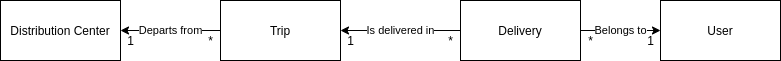
\includegraphics[scale=0.5]{thesis_svava/images/relations.png}}
    \caption{Relations of the different resources.}
    \label{fig:relations}
\end{figure}

\section{Architecture}
\begin{figure}
    \centerline{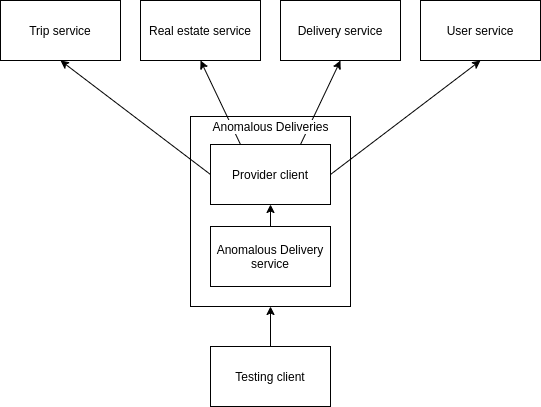
\includegraphics[scale=0.5]{thesis_svava/images/architecture.png}}
    \caption{The architecture for each service.}
    \label{fig:architecture}
\end{figure}

Each service implemented 5-6 methods/endpoints for fetching the data. These methods were based on the existing methods in the four Picnic microservices:
\begin{itemize}
    \item \texttt{getDeliveryById}: Accepts a single string parameter, returns a Delivery.
    \item \texttt{getDeliveryIdsByTripId}: Accepts a single string parameter, returns a list of strings.
    \item \texttt{getDistributionCenterById}: Accepts a single string parameter, returns a DistributionCenter.
    \item \texttt{getUserById}: Accepts a single string parameter, returns a User.
    \item \texttt{getTrips}: Accepts two date-time objects and a string, returns a list of Trips with a matching distributionCenterId which have a start time which falls between the two time instances supplied.
\end{itemize}
In addition, REST, RSocket and gRPC also implemented a sixth method:
\begin{itemize}
    \item \texttt{getTripOverviews}: Same parameters as \texttt{getTrips}, but returns a list of \texttt{TripOverviews}. Each \texttt{TripOverview} has all the same fields as a Trip, as well as a list of \texttt{DeliveryOverviews}. Similarly, each \texttt{DeliveryOverview} has the same fields as a \texttt{Delivery}, as well as a field for the respective User.
\end{itemize}
This method allows the other three services to fetch a collection of trips, the deliveries associated with them and the users associated with the deliveries, in a single request. The same was not needed for GraphQL, since GraphQL allows clients to specify which fields are needed, so \texttt{Deliveries} and \texttt{Users} can be included or omitted without any change in which method is called.

GraphQL and gRPC both offer the option of defining the set of fields in a resource deemed relevant for clients; GraphQL through its schema and gRPC through the proto file. Thus, for all resources the expected size of returned resources should be much smaller than for RSocket and REST. As an example, the \texttt{User} Java class imported from the Picnic ecosystem and returned in full by REST and RSocket contains 24 fields of types ranging from primitive (string), to complex, to sets of either type. In contrast, GraphQL and gRPC each only return 4 fields of a user, the \texttt{userId}, \texttt{firstname}, \texttt{lastname} and \texttt{contactEmail}.

\section{Implementation and deployment}
The services were all developed in Java Spring. That is both the technology of choice within Picnic, as well as convenient since a Spring Boot configuration already existed for each of the four communication methods. Efforts were made to keep the development of each service as homogeneous as possible, to ensure the performance was only affected by the specifics of each communication protocol/style. This included using Reactor for any reactive components, Jackson for serializing JSON (except for gRPC, which uses protocol buffers) and (where possible) using the same Java objects for the same resource (usually the ones defined in the existing microservices of Picnic). GraphQL and REST both use the Spring Webflux framework for HTTP communication and all four services use Netty as the server framework. 

Each service was wrapped in a Docker container and deployed to a Kubernetes cluster, to mimic the setup of a typical service within Picnic. The same configuration was used for each one to make sure no external variables affected their performance. 